% Method figure for v3-pure (fig_mm_v3_arch.pdf) — the working annotation-free loop.
% Companion to fig_af_rl_arch (the v1 recipe); same blue/orange convention:
%   BLUE = trainable retrieval path, ORANGE = frozen reward path.
%
% REPRO(fig:mm-v3-arch): both artifacts come from ONE layout spec so they cannot drift:
%   MMRAG_DATA=<data> python3 mmrag/plot_v3_arch.py --out mmrag/fig_mm_v3_arch
% It emits the edge-trimmed PDF (bbox_inches=tight) AND the editable fig_mm_v3_arch.pptx.
% Every hyperparameter on the figure is read from $MMRAG_DATA/runs/v3-pure/args.json at draw
% time — a missing key is a hard error, and the script refuses to draw a run that is not
% v3-pure (asserts algo=plgrpo, contrastive_coef=0, no_force_gold). The backbone name is parsed
% out of encoder.py:ENCODER_PROFILES, NOT derived from the reader (an earlier draft printed
% "Qwen2.5-VL-2B" for what is a Qwen2-VL encoder). A renderer bbox check measures every text
% extent against its owning box and reports violations; current status 0.
%
% NOTE the PDF is drawn by matplotlib from the shared spec rather than converted from the PPTX:
% this machine has no LibreOffice/soffice/unoconv. Re-export the PPTX through PowerPoint if a
% literally-converted PDF is wanted; the geometry is identical because both come from build_spec().
%
% Box -> code (VLM2Vec-rl @ v23-base): query/index train_rl.build_rl_corpus + refresh_corpus();
% policy encoder.load_encoder + rl_core.pool_logps; sampling rl_core.pl_sample_lists /
% pl_list_logps; reward reader_vlm.score_judge -> answer_correct; credit train_rl.main
% (R.mean over the list, z-score over G) + rl_core.embedding_ppo_loss.
\begin{figure}[t]
\centering
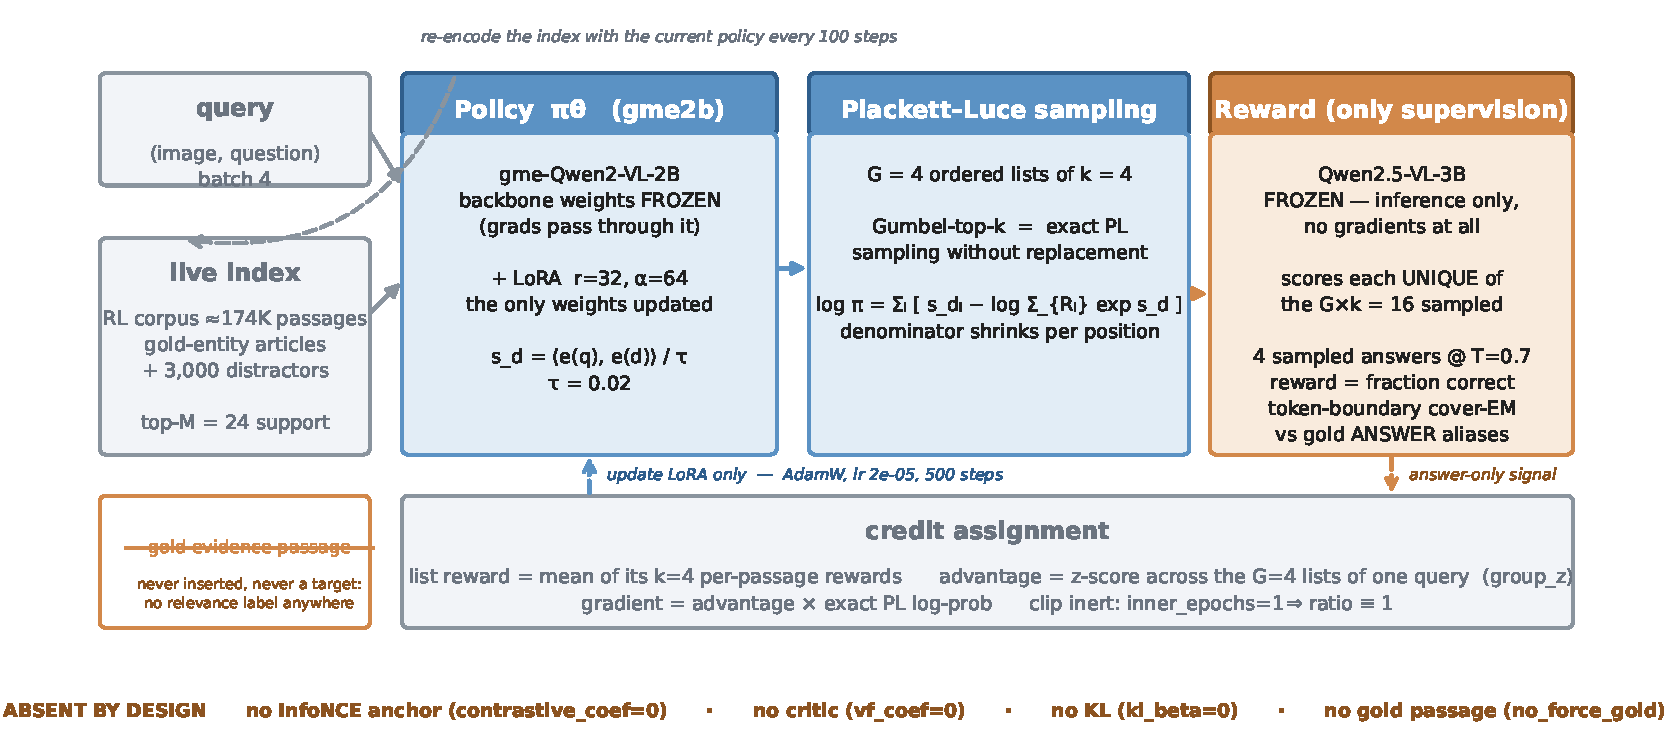
\includegraphics[width=\linewidth]{fig_mm_v3_arch.pdf}
\caption{\textbf{Training architecture of \textsc{v3-pure}, the working annotation-free loop.}
The retriever policy $\pi_\theta$ (\textsc{GME-Qwen2-VL-2B}; LoRA $r{=}32$, $\alpha{=}64$ are the
only trainable parameters) scores an image--question query against a \emph{live} index that is
re-encoded with the current policy every $100$ steps. An action is an ordered list of $k{=}4$
passages; $G{=}4$ such lists are drawn per query by Gumbel-top-$k$ over the policy's own top-$24$
support, which is exact Plackett--Luce sampling without replacement, and scored by the exact
conditional factorisation whose denominator shrinks at each position. A \emph{frozen}
\textsc{Qwen2.5-VL-3B} reader scores each unique sampled passage once, sampling $4$ answers at
$T{=}0.7$; the reward is the fraction that match a gold answer alias under token-boundary
cover-EM. List rewards are $z$-scored across the $G$ lists of a query, and the update is the
advantage-weighted exact log-probability --- with one inner epoch the PPO ratio is identically
one, so the clip never engages. Blue marks the trainable retrieval path, orange the frozen reward
path. What is \emph{absent} is the method's point: no InfoNCE anchor, no critic, no KL penalty,
and no gold passage --- the annotated evidence passage is never inserted into a pool and is never
a target, so the only supervision anywhere in the loop is the gold \emph{answer} string inside
the reward. Every hyperparameter shown is read from the shipped run's \texttt{args.json}; an
editable copy ships as \texttt{fig\_mm\_v3\_arch.pptx}.}
\label{fig:mm-v3-arch}
\end{figure}
